\section{\texorpdfstring{Construction of weight coefficients set $\Q$}{Construction of weight coefficients set Q}}
\label{app:phase1}   

\foreach \n in {1,...,13} {%
\begin{SCfigure}[][htbp]
    \centering
    \caption{Construction of the~weight coefficients set $\Q$ for Eisenstein numeration system}
    \label{img:phase1img\n}
    \includegraphics[height=0.3\textheight]{img/eisenstein/phase1_image_\n.png}
\end{SCfigure}
    }

\newpage
\section{\texorpdfstring{Construction of set $\Q_{[\omega,1,2]}$}{Construction of set Q[omega,1,2] for Eisenstein numeration system}}
\label{app:phase2}    
\foreach \n in {1,...,7} {%
\begin{SCfigure}[][htbp]
    \centering
    \caption{Construction of the set $\Q_{[\omega,1,2]}$ for Eisenstein numeration system}
    \label{img:phase2img\n}
    \includegraphics[height=0.3\textheight]{img/eisenstein/phase2_image_\n.png}
\end{SCfigure}
    }
    
    
% \begin{figure}[!htbp]
%   \centering
%   \begin{minipage}[b]{0.45\textwidth}
%     \FPeval{\numberImg}{clip(2*\n-1)}
%     \includegraphics[height=0.3\textheight]{img/eisenstein/phase1_image_\numberImg.png}
%     \caption{ }
%   \end{minipage}
%   \hfill
%   \begin{minipage}[b]{0.45\textwidth}
%     \FPeval{\numberImg}{clip(2*\n)}
%     \includegraphics[height=0.3\textheight]{img/eisenstein/phase1_image_\numberImg.png}
%     \caption{ }
%   \end{minipage}
% \end{figure}
%         \vfill


\newpage
\section{Sample of input file for shell}
File \verb+input_sample.sage+:
\label{app:inputSample}

\lstinputlisting[language=Python]{input_sample.sage}

\section{Interact in SageMath Cloud}
\label{app:interact}
\begin{figure}[!htbp]
  \centering
  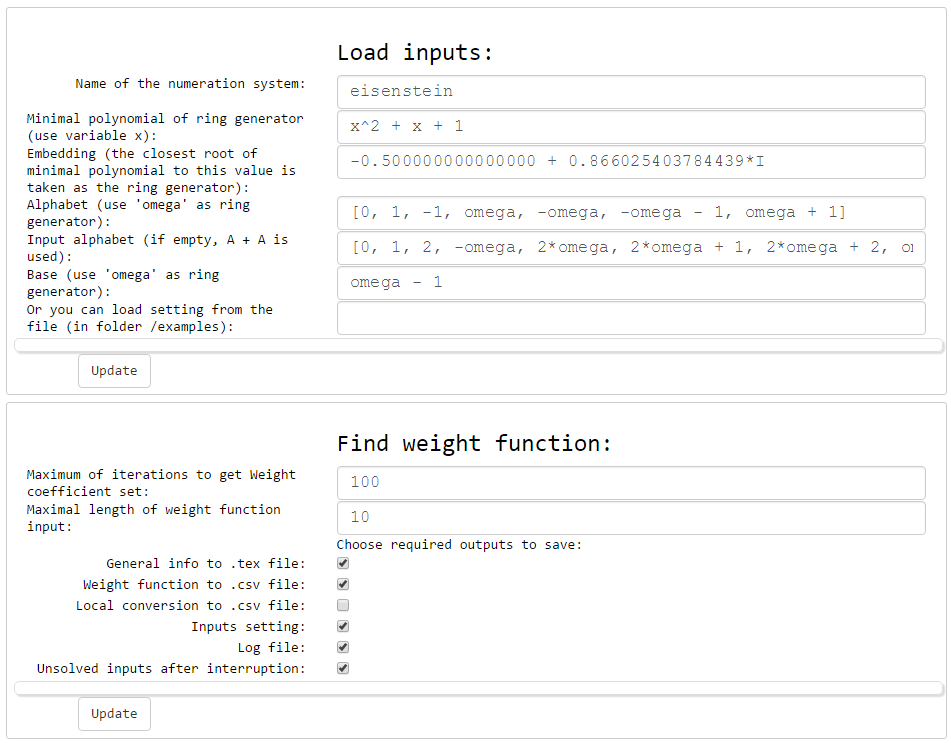
\includegraphics[width=\textwidth]{img/interact1.png}
  \caption{The interact after loading inputs.}
  \label{fig:interact1}
\end{figure}

\begin{figure}[htbp]
  \centering
  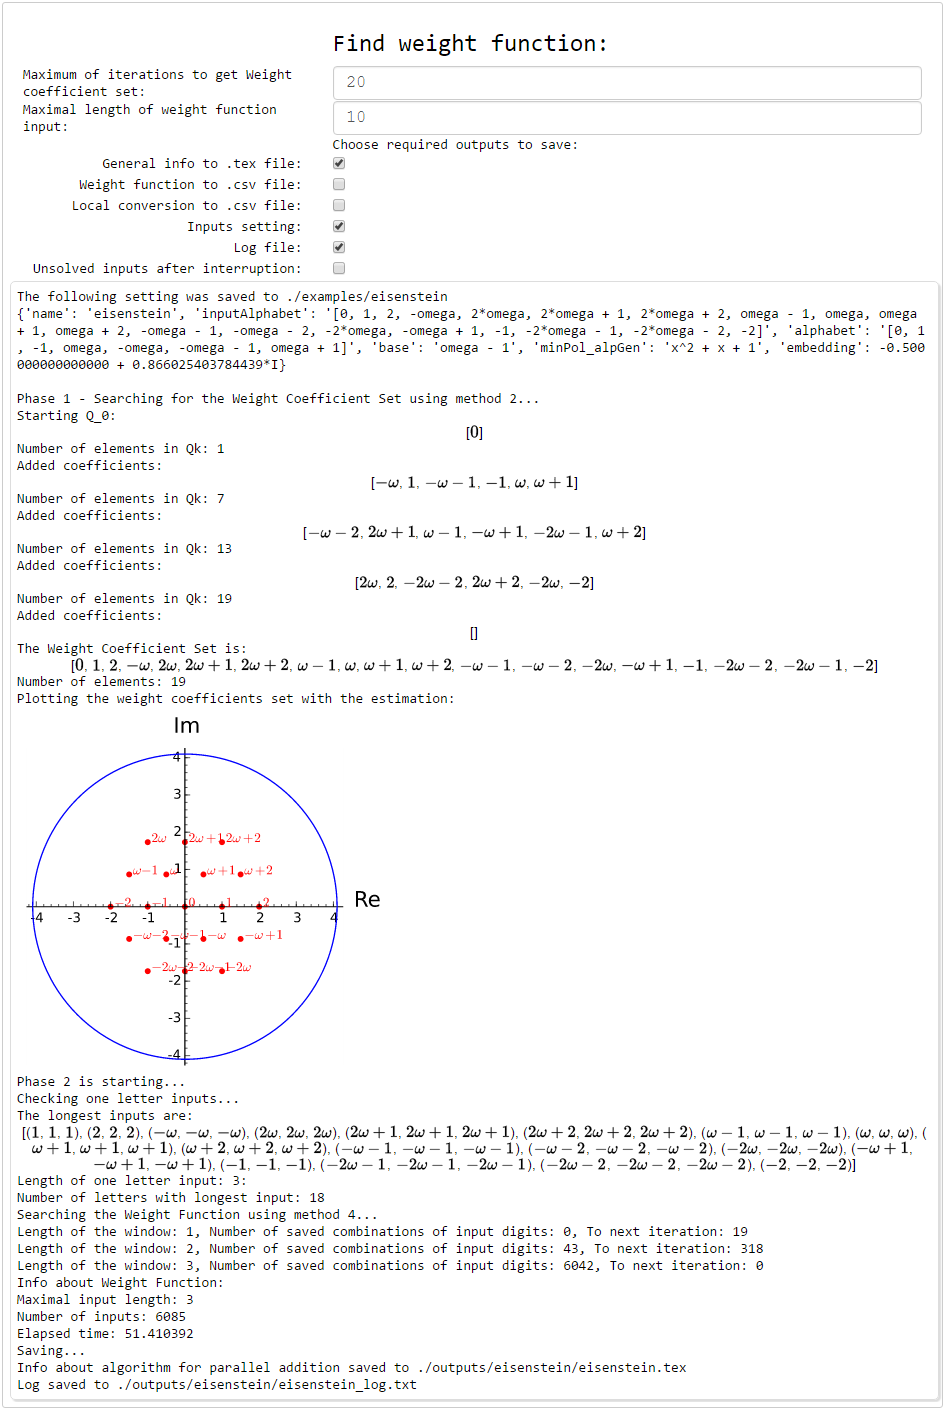
\includegraphics[width=\textwidth]{img/interact2.png}
  \caption{The output of the extending window method in the interact}
  \label{fig:interact2}
\end{figure}

\begin{figure}[htbp]
  \centering
  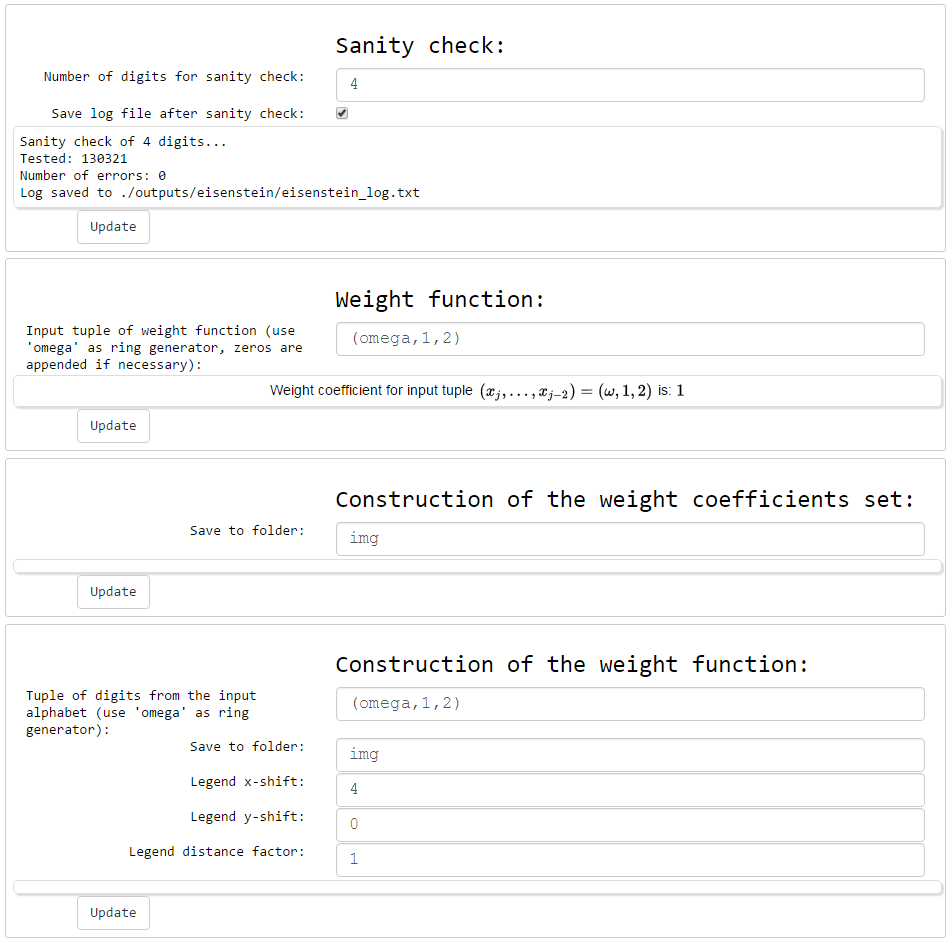
\includegraphics[width=\textwidth]{img/interact3.png}
  \caption{The part of the interact for the sanity check, calling of the weight function and plotting of images of steps of both phases.}
  \label{fig:interact3}
\end{figure}